\section{Gaussian Assumption Analysis}

\subsection*{What can you conclude on the goodness of the Gaussian assumption?}
The goodness of the Gaussian assumption varies significantly across the dataset's features. While the model correctly assumes that the data can be represented by a symmetric, bell-shaped probability density function for the majority of the feature space, it fundamentally fails to capture the true underlying empirical distribution of data that exhibits strong asymmetry. Therefore, the overall assumption is only partially valid for this dataset.

\subsection*{Is it accurate for all the 6 features?}
No, the Gaussian assumption is not accurate for all 6 features. It is only accurate for the first four features (Features 1, 2, 3, and 4). These specific features naturally exhibit a roughly symmetric, normal distribution, meaning the mathematical Gaussian curve maps to their empirical densities quite well.

\subsection*{Are there features for which the assumptions do not look good?}
Yes, the assumption does not look good at all for Features 5 and 6. Both of these features are heavily skewed, characterized by a sharp peak concentrated on one side and a long trailing tail on the other. Because a Gaussian distribution is strictly symmetric around its mean, it cannot bend to fit these skewed shapes. Consequently, the model drastically underestimates the true density at the core peaks and overestimates the density on the steep drop-offs.

\begin{figure}[H]
    \centering
    % Row 1
    \begin{subfigure}{0.48\textwidth}
        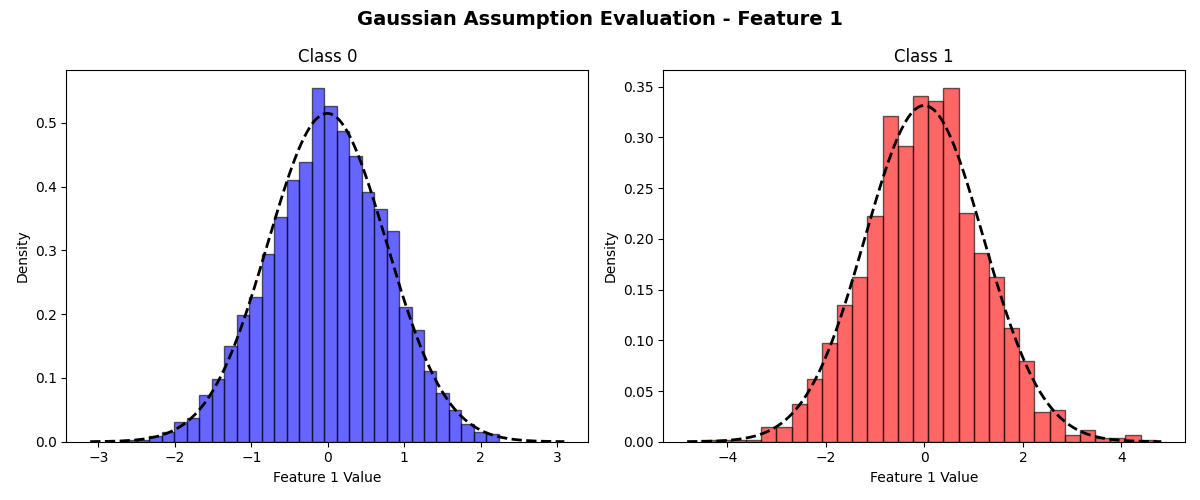
\includegraphics[width=\linewidth]{images/feature_1_distribution.png}
        \caption{Feature 1 (Good Fit)}
    \end{subfigure}\hfill
    \begin{subfigure}{0.48\textwidth}
        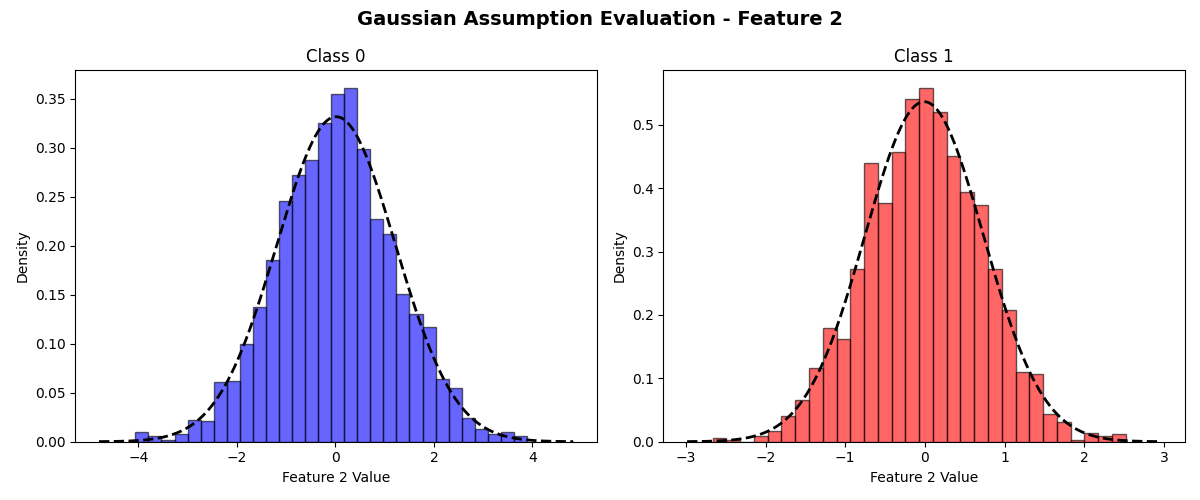
\includegraphics[width=\linewidth]{images/feature_2_distribution.png}
        \caption{Feature 2 (Good Fit)}
    \end{subfigure}
    
    \vspace{0.5cm}
    % Row 2
    \begin{subfigure}{0.48\textwidth}
        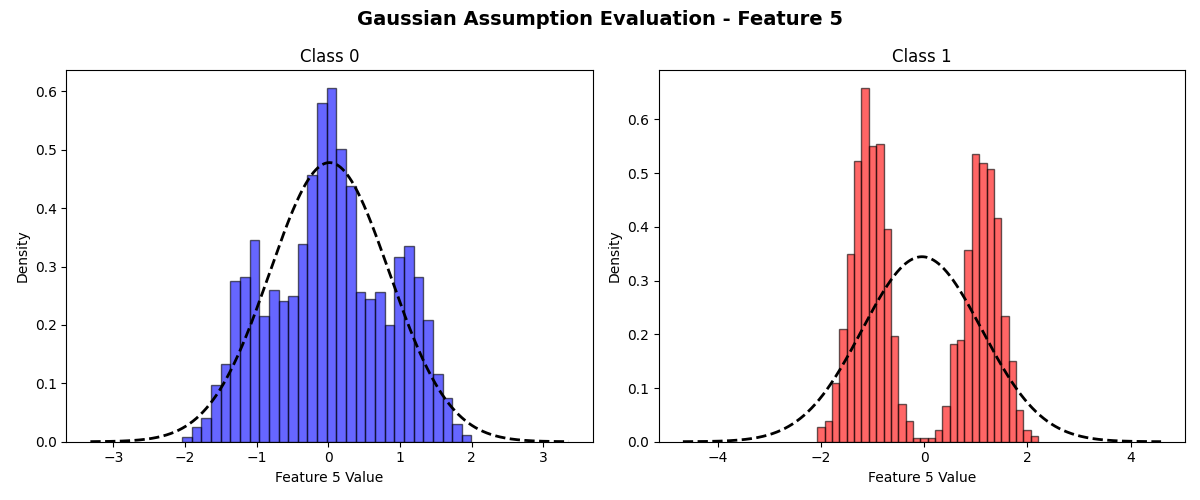
\includegraphics[width=\linewidth]{images/feature_5_distribution.png}
        \caption{Feature 5 (Poor Fit - Skewed)}
    \end{subfigure}\hfill
    \begin{subfigure}{0.48\textwidth}
        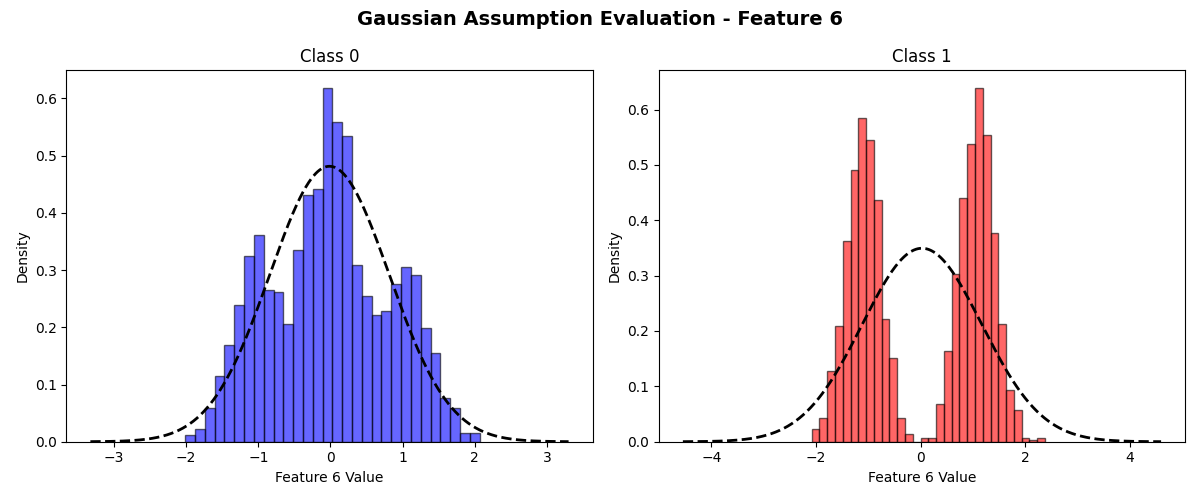
\includegraphics[width=\linewidth]{images/feature_6_distribution.png}
        \caption{Feature 6 (Poor Fit - Skewed)}
    \end{subfigure}
    \caption{Comparison of features that adhere well to the Gaussian assumption (top) versus features that severely violate it due to skewness (bottom).}
    \label{fig:gaussian_fits}
\end{figure}